\documentclass[a4paper,11pt]{article}
%\documentclass[a4paper,11pt,twocolumn]{article}%twocolumn layout; not sure if this works correctly. Feel free to experiment.
\usepackage[pdftex]{color,graphicx}
\usepackage[T1]{fontenc}
\usepackage{amsmath} %must be loaded before pxfonts, otherwise \iint is defined twice
\usepackage{pxfonts}
\usepackage{subfigure}
\usepackage{xcolor}

%color links to figs, etc.
%\usepackage[pdftex,colorlinks,urlcolor=blue,breaklinks]{hyperref}
\usepackage[pdftex,colorlinks]{hyperref}
\hypersetup{colorlinks,%
		    citecolor=black,%
		    filecolor=black,%
		    linkcolor=black,%
		    urlcolor=black,%
		    breaklinks=true,%
		    pdftex}

%easily manipulate margins
\usepackage{geometry}
\makeatletter
\if@twocolumn%
	\geometry{twoside,
		paperwidth=210mm,
  		paperheight=297mm,
  		textheight=682pt,
  		textwidth=516pt,
  		centering,
  		headheight=50pt,
  		headsep=12pt,
  		footskip=18pt,
  		footnotesep=24pt plus 2pt minus 12pt,
 		columnsep=14pt}
\else%if using twocolumns, I still need to modify the textwidth to accomodate the watermark
	\geometry{twoside,
		  paperwidth=210mm,
		  paperheight=297mm,
		  textheight=750pt,
		  textwidth=500pt,
		  centering,
		  headheight=50pt,
		  headsep=12pt,
		  footskip=18pt,
		  footnotesep=24pt plus 2pt minus 12pt}
\fi%

%change the font
\usepackage{charter}

%CC logos to add in the footer
% \usepackage{ccicons}

%easily manipulate color
\usepackage{color}

\usepackage[utf8]{inputenc} % allow utf-8 input
\usepackage[T1]{fontenc}    % use 8-bit T1 fonts
\usepackage{hyperref}       % hyperlinks
\usepackage{url}            % simple URL typesetting
\usepackage{booktabs}       % professional-quality tables
\usepackage{amsfonts}       % blackboard math symbols
\usepackage{nicefrac}       % compact symbols for 1/2, etc.
\usepackage{microtype}      % microtypography
\usepackage{xcolor}         % colors
\usepackage{algorithmicx}
\usepackage{algorithm, algpseudocode}
\usepackage{graphicx}
\usepackage{adjustbox}
\usepackage{mathrsfs}

%nicely print bioRxiv
\newcommand{\biorxiv}{\emph{bio{\color{red}R}$\chi$iv}}

%add biorxiv type of article using the package background
\usepackage{tikz}
\usetikzlibrary{positioning,arrows.meta}
\usepackage[firstpage=True]{background}


\newcommand{\newresults}{
\makeatletter
\if@twocolumn%
	\backgroundsetup{
		position={0.572\paperwidth,-0.025\paperheight} ,
		angle=270,
		color=black,
		opacity=0.60,
		scale=1.5,
		contents={\tikz\node[text=black,fill=gray!40,align=left, minimum width=2.3cm,minimum height=0.6cm,inner sep=0]{New Results};}}
\else
	\backgroundsetup{
		position={0.338\paperwidth,-0.06\paperheight} ,
		angle=270,
		color=black,
		opacity=0.60,
		scale=2.5,
		contents={\tikz\node[text=black,fill=gray!40,align=left, minimum width=2.3cm,minimum height=0.6cm,inner sep=0]{New Results};}}
\fi%
}

\newcommand{\confirmatoryresults}{
\makeatletter
\if@twocolumn%
\backgroundsetup{
	position={0.572\paperwidth,-0.03\paperheight} ,
	angle=270,
	color=black,
	opacity=0.60,
	scale=1.5,
	contents={\tikz\node[text=black,fill=gray!40,align=left, minimum width=3.9cm,minimum height=0.6cm,inner sep=0]{Confirmatory Results};}}
\else
	\backgroundsetup{
	position={0.338\paperwidth,-0.07\paperheight} ,
	angle=270,
	color=black,
	opacity=0.60,
	scale=2.5,
	contents={\tikz\node[text=black,fill=gray!40,align=left, minimum width=3.9cm,minimum height=0.6cm,inner sep=0]{Confirmatory Results};}}
\fi%
}

\newcommand{\contradictoryresults}{
\makeatletter
\if@twocolumn%
	\backgroundsetup{
	position={0.572\paperwidth,-0.03\paperheight} ,
	angle=270,
	color=black,
	opacity=0.0,
	scale=1.5,
	contents={\tikz\node[text=black,fill=gray!40,align=left, minimum width=4.0cm,minimum height=0.6cm,inner sep=0]{};}}
\else
	\backgroundsetup{
	position={0.338\paperwidth,-0.07\paperheight} ,
	angle=270,
	color=black,
	opacity=0.0,
	scale=2.5,
	contents={\tikz\node[text=black,fill=gray!40,align=left, minimum width=4.0cm,minimum height=0.6cm,inner sep=0]{};}}
\fi%
}

%enhanced floats
\usepackage{float}

%rotate floats if necessary
\usepackage{rotating}

%nicer, clever tables, uncomment if necessary
\usepackage{supertabular}

%tables with notes, etc., uncomment if necessary
%\usepackage{threeparttable}

%improved captions, uncomment if necessary
\usepackage{caption}

%add an author block
\usepackage{authblk}
%redefine authorblock font size and affiliation font size
\renewcommand\Authfont{\small}
\renewcommand\Affilfont{\scriptsize}

%add nice headers
\usepackage{fancyhdr}
\pagestyle{fancy}
\renewcommand{\headrulewidth}{0pt}
\lhead{{\footnotesize }}
\chead{}
\rhead{{\footnotesize }}
% \lfoot{}
\cfoot{\thepage}
% \rfoot{\biorxiv}


\usepackage{draftwatermark}
\makeatletter
\if@twocolumn
	\SetWatermarkText{}
	\SetWatermarkScale{0.20}
	\SetWatermarkAngle{270}
	%note: I defined this commands in the draftwatermark.sty file. For some reason they are in teh manual but not in the sty file...
	\SetWatermarkHorCenter{0.97\paperwidth}
	\SetWatermarkVerCenter{-.88\paperheight}
\else
	\SetWatermarkText{}
	\SetWatermarkScale{0.25}
	\SetWatermarkAngle{270}
	%note: I defined this commands in the draftwatermark.sty file. For some reason they are in teh manual but not in the sty file...
	\SetWatermarkHorCenter{0.95\paperwidth}
	\SetWatermarkVerCenter{-.82\paperheight}
\fi

%uncomment the type of bioRxiv preprint below to added to the first page
%\newresults{}
%\confirmatoryresults{}
\contradictoryresults{}

%flushleft the title, authorblock and Abstract
%modified from http://tex.stackexchange.com/questions/85343/left-align-abstract-title-and-authors
\makeatletter
\renewcommand{\maketitle}{\bgroup\setlength{\parindent}{0pt}
\begin{flushleft}
  \thispagestyle{plain}
  \textbf{\@title}

  \@author
\end{flushleft}\egroup
}
\makeatother

%redefine the abstract
\renewenvironment{abstract}
 {\small
  \begin{flushleft}
  \textbf{\abstractname}\vspace{-0.40em}\vspace{0pt}
  \end{flushleft}
  \list{}{
    \setlength{\leftmargin}{0cm}%
    \setlength{\rightmargin}{\leftmargin}%
  }%
  \item\relax}
 {\endlist}

\hyphenation{}

\renewcommand*{\thefootnote}{\fnsymbol{footnote}}

%if to do notes need to be added: need to configure this!
\usepackage[colorinlistoftodos]{todonotes}
% \fillin marks every value only the authors can supply (red in the PDF). Search for it before submitting.
\newcommand{\fillin}[1]{{\color{red}[#1]}}

%feel free to change the reference style to suit your needs
\usepackage[firstinits=true, backref=false, maxcitenames=1,  hyperref=auto, style=authoryear, defernumbers=true, backend=bibtex]{biblatex}[2010/11-19]

\usepackage{filecontents}
\begin{filecontents*}{Literature.bib}
@misc{kaggle2026constellation,
  title={Constellation Detection - {CS-GY} 6643},
  author={Mishra, Akshat and Pandey, Anushk and {DipeshK27} and Viegas, Thiago},
  howpublished={\url{https://www.kaggle.com/competitions/constellation-detection-cs-gy-6643}},
  note={Kaggle},
  year={2026}
}
@article{lowe2004distinctive,
  title={Distinctive image features from scale-invariant keypoints},
  author={Lowe, David G.},
  journal={International Journal of Computer Vision},
  volume={60}, number={2}, pages={91--110}, year={2004}
}
@article{fischler1981ransac,
  title={Random sample consensus: a paradigm for model fitting with applications to image analysis and automated cartography},
  author={Fischler, Martin A. and Bolles, Robert C.},
  journal={Communications of the ACM},
  volume={24}, number={6}, pages={381--395}, year={1981}
}
@article{torr2000mlesac,
  title={{MLESAC}: A new robust estimator with application to estimating image geometry},
  author={Torr, Philip H. S. and Zisserman, Andrew},
  journal={Computer Vision and Image Understanding},
  volume={78}, number={1}, pages={138--156}, year={2000}
}
@article{umeyama1991least,
  title={Least-squares estimation of transformation parameters between two point patterns},
  author={Umeyama, Shinji},
  journal={IEEE Transactions on Pattern Analysis and Machine Intelligence},
  volume={13}, number={4}, pages={376--380}, year={1991}
}
@inproceedings{lewis1995fast,
  title={Fast normalized cross-correlation},
  author={Lewis, J. P.},
  booktitle={Vision Interface},
  pages={120--123}, year={1995}
}
@article{groth1986pattern,
  title={A pattern-matching algorithm for two-dimensional coordinate lists},
  author={Groth, Edward J.},
  journal={The Astronomical Journal},
  volume={91}, pages={1244--1248}, year={1986}
}
@article{lang2010astrometry,
  title={Astrometry.net: Blind astrometric calibration of arbitrary astronomical images},
  author={Lang, Dustin and Hogg, David W. and Mierle, Keir and Blanton, Michael and Roweis, Sam},
  journal={The Astronomical Journal},
  volume={139}, number={5}, pages={1782--1800}, year={2010}
}
@article{bertin1996sextractor,
  title={{SExtractor}: Software for source extraction},
  author={Bertin, Emmanuel and Arnouts, St{\'e}phane},
  journal={Astronomy and Astrophysics Supplement Series},
  volume={117}, pages={393--404}, year={1996}
}
@article{stetson1987daophot,
  title={{DAOPHOT}: A computer program for crowded-field stellar photometry},
  author={Stetson, Peter B.},
  journal={Publications of the Astronomical Society of the Pacific},
  volume={99}, pages={191--222}, year={1987}
}
@article{lindeberg1998feature,
  title={Feature detection with automatic scale selection},
  author={Lindeberg, Tony},
  journal={International Journal of Computer Vision},
  volume={30}, number={2}, pages={79--116}, year={1998}
}
@article{rousseeuw1993alternatives,
  title={Alternatives to the median absolute deviation},
  author={Rousseeuw, Peter J. and Croux, Christophe},
  journal={Journal of the American Statistical Association},
  volume={88}, number={424}, pages={1273--1283}, year={1993}
}
@misc{cv2026lectures,
  title={{CS-GY} 6643 Computer Vision, Lectures 1--3},
  author={{NYU Tandon}},
  note={Course slides, Fall 2026},
  year={2026}
}
\end{filecontents*}
\bibliography{Literature}

\newcommand{\yz}[1]{{\color{blue}[Yizi: #1]}}

\definecolor{dodgerblue}{rgb}{0.12, 0.56, 1.0}
\definecolor{lightseagreen}{rgb}{0.13, 0.7, 0.67}
\definecolor{mediumorchid}{rgb}{0.73, 0.33, 0.83}
\definecolor{electriclavender}{rgb}{0.96, 0.73, 1.0}
\definecolor{royalazure}{rgb}{0.0, 0.22, 0.66}
\definecolor{cadetgrey}{rgb}{0.57, 0.64, 0.69}
\definecolor{applegreen}{rgb}{0.55, 0.71, 0.0}
\definecolor{darkpastelpurple}{rgb}{0.59, 0.44, 0.84}
\definecolor{purpleheart}{rgb}{0.41, 0.21, 0.61}



\begin{document}

%always keep the \newline command at the end of the title to add space between the title and the authors
\title{\Large CS-GY 6643 Computer Vision -- Project 1, Kaggle Competition Report
\newline}
\author{Rushil Aramandla, ra4880@nyu.edu, \fillin{Teammate name}, \fillin{netid}@nyu.edu}


\date{}

\maketitle
%\tableofcontents

\noindent
\textbf{Kaggle team name:} Merchants Of San Ramon \fillin{check the exact spelling on the leaderboard}\\

\section{Introduction and background}

\paragraph{Task.} The competition \parencite{kaggle2026constellation} gives a set of \emph{scenes}. Each scene is a
$3000\times3000$ 8-bit grayscale sky image and a folder of $32\times32$ 8-bit query patches (``tiles''), 21 to 87 per
scene. Every tile is one of three kinds, and we are never told which: a star of the constellation figure the scene
depicts, another real star of the same sky (off-figure), or a crop from a different sky (absent). For every tile we
report either $-1$ (absent) or $(x, y, m)$, the tile centre's position in the sky with $m=1$ if we claim it is a figure
star. For every scene we name one of 48 reference constellations, supplied as line drawings in \texttt{patterns/}. Each
scene is scored independently and the scores are averaged:
\begin{equation}
S = 0.25\,\mathrm{Presence} + 0.20\,\mathrm{Localization} + 0.25\,\mathrm{GeometricRecovery} + 0.30\,\mathrm{Identification}.
\end{equation}
Presence is the macro-F1 of the present/absent decision. Localization is the mean reward over truly present tiles:
full credit within 12\,px, zero at 36\,px and beyond, linear in between. GeometricRecovery matches the issued figure
stars one-to-one to all reported present points under the same ramp. Identification is 1 for the exact name and 0
otherwise.

\paragraph{Why it is hard.} Presence and name together carry 55\% of the score, and both need a global
geometric argument, not a local one.
\begin{itemize}
\item \emph{Self-similarity.} A $32\times32$ window holds a few anonymous point sources, and thousands of other places in
the sky look much the same. There is no texture, colour or semantics to match.
\item \emph{Degradations.} Each tile is rotated by an arbitrary angle, rescaled, shifted by a fraction of a pixel,
blurred, dimmed or brightened by a smooth illumination drift, noised and JPEG-compressed. Only the tile centre is
preserved. The skies are real survey mosaics with seams, nebulosity, saturated stars and diffraction spikes. The
noise level also varies a lot between scenes (the robust noise we measure ranges from about 4.5 to 22 grey levels).
\item \emph{Bright stars.} A saturated tile is a round flat blob. It correlates at $\geq0.95$ with every other bright
star in the sky, so the textbook best-correlation peak is often the wrong star (Section~\ref{sec:method}).
\item \emph{Contaminated, partial geometry.} Only some of a figure's stars are issued as tiles. Off-figure stars sit in
the same pile, and neighbouring real constellations appear as decoys (e.g.\ Orion's stars inside the Taurus training
sky). The drawings are schematics: their scale, orientation, handedness and aspect ratio are unrelated to the sky.
\item \emph{Very little labelled data.} There are three labelled training scenes (116 tiles) and 16 unlabelled
validation scenes. The hidden scenes may depict constellations that do not appear in training, which rules out
learning a per-constellation classifier.
\end{itemize}

\paragraph{Prior work.} Locating a tile is template matching by normalised cross-correlation (NCC) \parencite{lewis1995fast},
covered in Lecture~1 together with smoothing, median filtering and histograms \parencite{cv2026lectures}. Making it
work under rotation and scale is the problem SIFT-style keypoints and descriptors solve \parencite{lowe2004distinctive}
(Lecture~2). Lowe's ratio test is the standard way to reject ambiguous matches. Naming the figure is point-set
registration under heavy outlier contamination. The usual tools are hypothesise-and-verify with RANSAC
\parencite{fischler1981ransac} (Lecture~3), least-squares similarity fitting \parencite{umeyama1991least}, and
likelihood-based scoring of hypotheses as in MLESAC \parencite{torr2000mlesac}. In astronomy this is \emph{plate
solving}. Triangle matching of star lists \parencite{groth1986pattern} and Astrometry.net's geometric hashing of star
quads with a Bayesian verification step \parencite{lang2010astrometry} solve it blind. Star detection and photometry
use matched filtering and robust background estimation \parencite{stetson1987daophot, bertin1996sextractor}.

\paragraph{Our approach.} We built a classical, training-free plate solver (no learned weights). It extracts a star catalogue from the
sky, locates every tile with a rotation/zoom correlation sweep and a halo-free verification correlation, and decides
presence with a ratio-test-style rule. It names the constellation by fitting every drawing to the brightest stars with
exhaustive two-point similarity hypotheses. Each fit is scored by a log-likelihood ratio and calibrated against
scrambled copies of the same drawing. Finally it places unresolved bright tiles on the named figure's stars. We
expected this to work for three reasons. The only reliable signal is geometry. Every constant can be expressed in
pixels or noise units, so nothing depends on a particular scene. And, as we measured on the training scenes, the
figure is a similarity transform of the drawing whose stars are among the brightest in the image.

\textbf{Credit.} The structure of the final pipeline (bright-star naming with a likelihood score and a scrambled-figure
null, figure-guided placement of bright tiles) was adapted from a classmate's solution to the same competition, which
we studied and then re-implemented and restructured. \fillin{Name the classmate, or confirm with the instructor how to
credit them.} Our own earlier pipelines are described in Section~\ref{sec:alternatives}.

\section{Datasets}

\subsection{Preprocessing}

\paragraph{Data.} Table~\ref{tab:data} summarises the data. The three training scenes (Pisces, Scorpius, Taurus) have
41, 41 and 34 tiles. Absent tiles are 34--47\% of each scene and figure stars only 18--24\%, so the classes are
imbalanced; the macro-F1 used for Presence partly offsets this. The 16 validation scenes hold 668 tiles (21--87 per
scene). We found no missing or corrupted files. Figure~\ref{fig:data} shows the data and every preprocessing stage.

\begin{table}[h]
\centering\small
\begin{tabular}{lrrrr}
\toprule
scene & tiles & figure ($m{=}1$) & off-figure ($m{=}0$) & absent \\
\midrule
train / pisces   & 41 & 10 & 17 & 14 \\
train / scorpius & 41 & 10 & 16 & 15 \\
train / taurus   & 34 &  6 & 12 & 16 \\
\midrule
validation (16 scenes, unlabelled) & 668 & -- & -- & -- \\
\bottomrule
\end{tabular}
\caption{\textbf{Label distribution.} Tile counts per training scene by class, from \texttt{train\_ground\_truth.csv}.
Validation labels are hidden.}
\label{tab:data}
\end{table}

\paragraph{Sky preprocessing} (in order):
\begin{enumerate}
\item \emph{Background removal.} The sky is shrunk $4\times$ by area averaging and median-filtered with a 31-px window
(about 124 full-resolution px). The result is upsampled bilinearly and subtracted. A median fits because stars are
sparse outliers on a piecewise-flat background of seams and nebulosity (Fig.~\ref{fig:data}b--d).
\item \emph{Despeckling.} A $3\times3$ median removes hot pixels before detection only.
\item \emph{Star detection.} A Gaussian filter ($\sigma=1.2$\,px) is the matched filter for a point source. Local maxima
above $3.6\hat\sigma$ survive, where $\hat\sigma = 1.4826\cdot\mathrm{MAD}$ is a robust noise estimate
\parencite{rousseeuw1993alternatives}. Non-maximum suppression uses dilation (radius 3). Position and flux come from
$5\times5$ intensity-weighted box sums. This gives 1.8k--9.5k stars per scene.
\item \emph{Saturated stars.} A blown-out star has a flat top, so its box centroid is unreliable. Such stars move to the
centroid of their compact saturated connected component ($\geq250$, $\geq3$ px, fill $\geq0.3$, which excludes seams
and spikes). Detections that share a plateau are merged. The saturated-pixel count in a $25\times25$ box is kept as a
brightness proxy.
\item \emph{Correlation image.} The background-free sky is smoothed ($\sigma=1$), divided by $\hat\sigma$, and mapped
through $\mathrm{sign}(x)\sqrt{|x|}$. This point transform keeps the brightness order but stops one saturated star from
dominating every correlation window (Fig.~\ref{fig:data}e--g). We did not use histogram equalisation, because it
destroys the brightness ratios the matching relies on.
\end{enumerate}

\paragraph{Tile preprocessing} (same steps at tile scale): subtract a 9-px median background followed by a Gaussian
($\sigma=3$) smooth, which removes the illumination drift; apply a $3\times3$ median; subtract the ring-average radial profile about the
centre so the central star's halo does not hide its neighbours; detect stars ($\sigma=1$, $3.2\hat\sigma$); and apply the
same $\mathrm{sign}\sqrt{\cdot}$ stretch. The star within 2.5\,px of the centre is the \emph{anchor}. Up to 8
neighbours (distance, angle, flux, SNR weight) form a small rotation-covariant descriptor. The radius at which the ring
profile falls below 25\% of the central excess is the \emph{halo radius}. A tile whose halo reaches 6\,px is a
\emph{bright-star tile} and is handled separately (Section~\ref{sec:method}).

\paragraph{Drawings.} The patterns are RGBA line art. Their star nodes are the white dots (alpha $>100$, all channels
$>150$): connected components of 4--400 px. Oversized or elongated blobs are split at the maxima of their distance
transform, and a fallback handles drawings without white dots. Each dot's area is kept, since larger dots mark
brighter stars. Nodes are normalised to zero mean and unit RMS radius, giving 2 to 28 nodes per figure.

\paragraph{Splits and augmentation.} No training happens, so there is no train/validation split in the usual sense and no
augmentation. The three labelled scenes serve only to check the pipeline and to set a handful of thresholds. The 16
validation scenes are the ones scored on Kaggle. The competition rules forbid scene-specific constants. Every
parameter is therefore a pixel, noise-unit or score quantity, and the code never reads scene names.

\begin{figure*}[h]
    \centering
    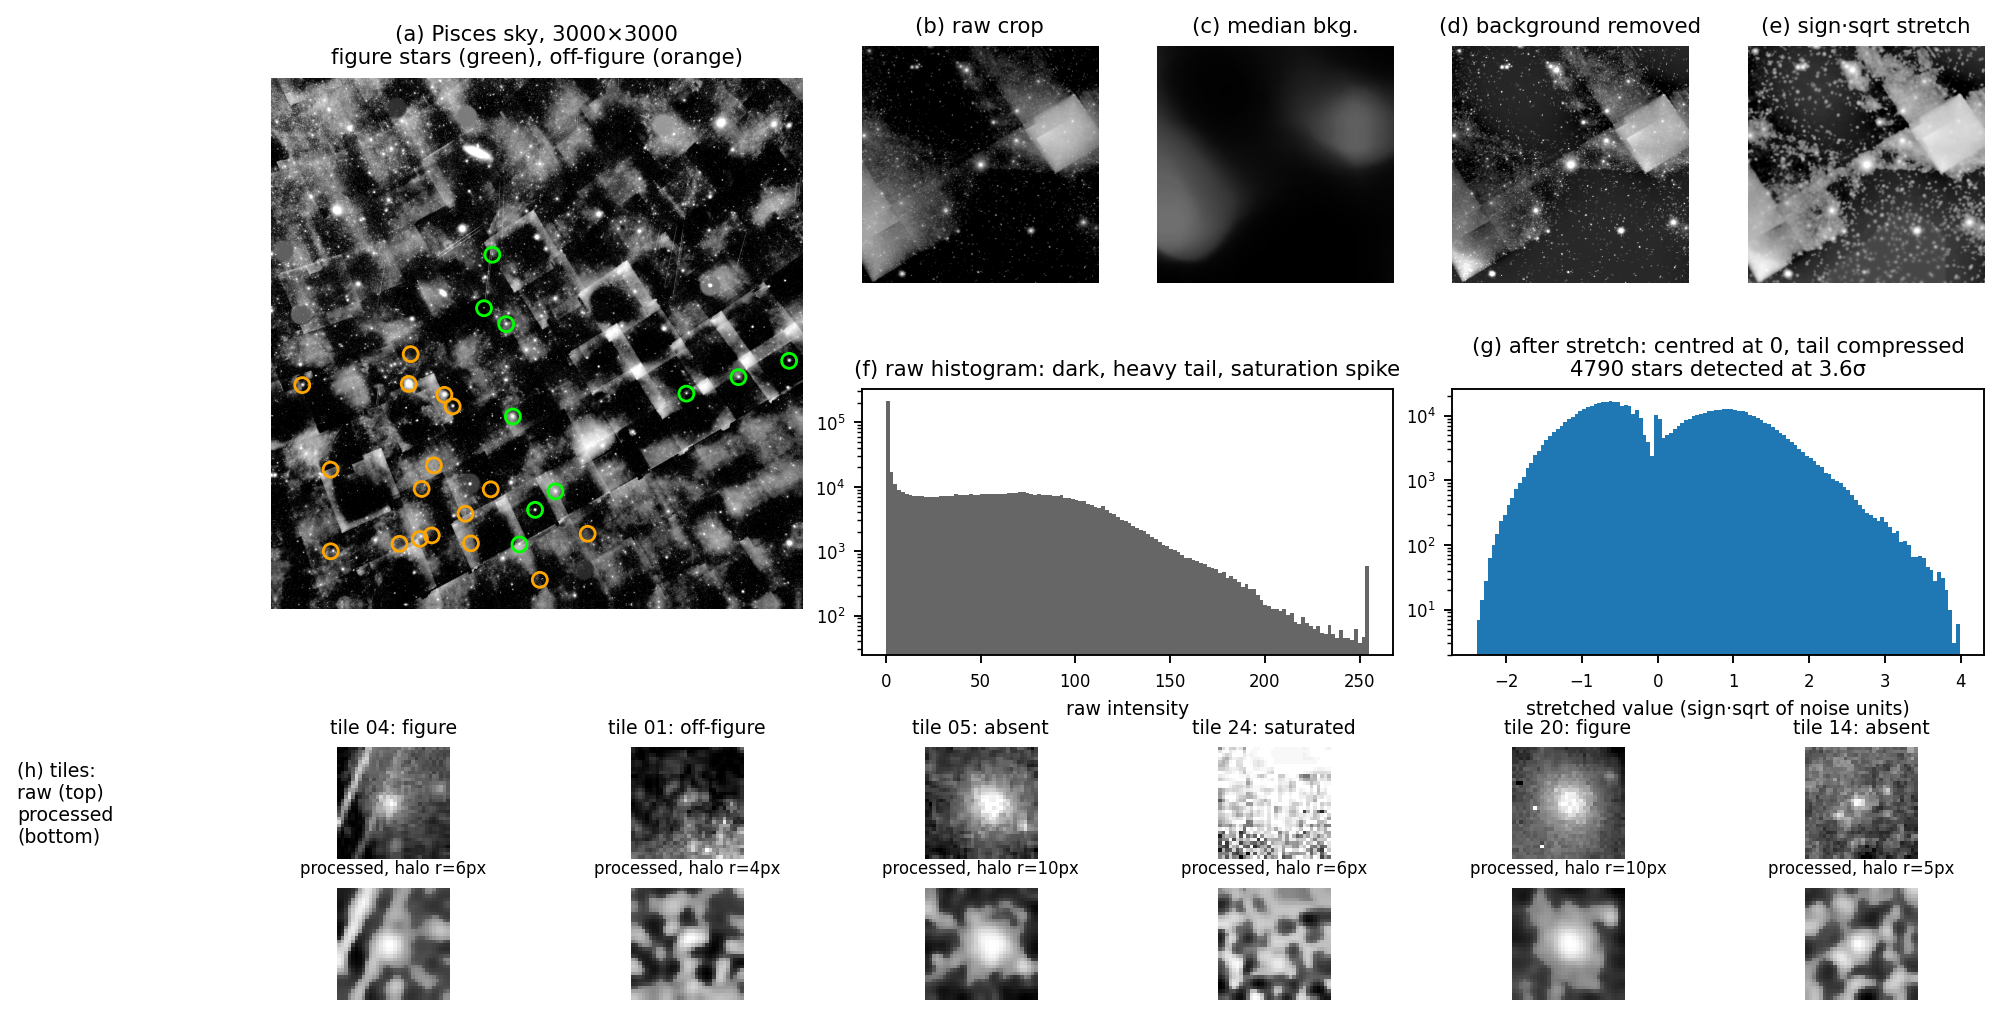
\includegraphics[width=\linewidth]{figs/preprocessing.png}
    \caption*{\textbf{Figure 1: the data and each preprocessing stage (Pisces training scene).} (a) The full
    $3000\times3000$ sky, with mosaic seams, nebulosity and a galaxy visible. Circles mark the labelled present tiles:
    green are figure stars, orange are off-figure stars. (b) A $300\times300$ crop around a figure star. (c) Its median
    background model. (d) The crop after background subtraction. (e) After Gaussian smoothing and the
    $\mathrm{sign}\sqrt{\cdot}$ stretch in robust-noise units, the representation used for correlation. (f) Histogram of
    the raw sky (log scale): most pixels are dark, with a long bright tail and a spike at saturation (255). (g) The same
    after preprocessing: centred on zero with the tail compressed; 4,790 stars are detected at $3.6\hat\sigma$.
    (h) Six query tiles, raw (top) and after tile preprocessing (bottom): figure, off-figure and absent tiles look
    alike, and the saturated tile (24) has no usable internal structure.}
    \label{fig:data}
\end{figure*}

\subsection{External and Auxiliary Datasets}
None. We used no external data, star catalogues or pretrained weights. The only inputs are the competition's
\texttt{participant/} folder (\texttt{patterns/}, \texttt{train/}, \texttt{validation/}, \texttt{sample\_submission.csv},
\texttt{train\_ground\_truth.csv}). The libraries used are NumPy, SciPy, OpenCV, scikit-image and PyTorch; PyTorch is
used only as a GPU convolution engine.

\section{Methods}
\label{sec:method}

\paragraph{Formulation.} For a scene with sky $I$, tiles $\{T_k\}$ and figures $\{\mathcal F_j\}_{j=1}^{48}$ (each a
normalised node set $\{u_{ji}\}$ with dot sizes), we estimate for every tile a pose $(x_k, y_k, \theta_k, s_k)$ and a
presence bit $\pi_k$. For the scene we estimate a figure index $j^\star$ and a transform $A,t$ that maps the drawing to
the sky. We optimise no loss by gradient descent. Each stage maximises an explicit score:
\begin{itemize}
\item tile pose: $\arg\max_{x,y,\theta,s}\ \mathrm{NCC}\big(\mathcal W_{\theta,s}(T_k),\ I_{x,y}\big)$ on the halo-free,
stretched images;
\item presence: a thresholded decision on the best NCC, its lead over the best competitor more than 5\,px away, and a
$z$-score of the best NCC against 200 random poses;
\item name: $j^\star = \arg\max_j\ \big[\max(\mathrm{LLR}_j,0) - \mu^{\mathrm{null}}_j - \sigma^{\mathrm{null}}_j\big]$,
where $\mathrm{LLR}_j$ is the best log-likelihood ratio of ``figure $j$ is here'' vs.\ ``these are random stars''
over all similarity/affine hypotheses.
\end{itemize}

\subsection{Proposed Method}

\begin{figure*}[h]
\centering
\begin{adjustbox}{width=\linewidth}
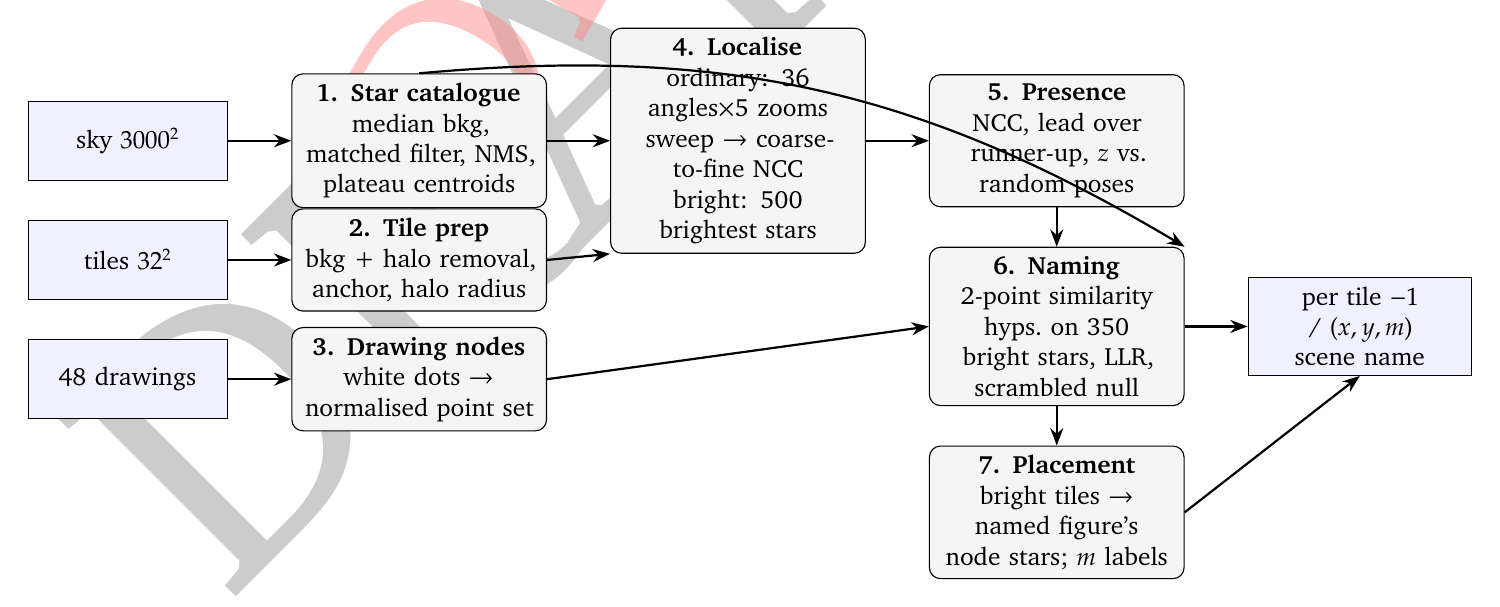
\begin{tikzpicture}[
  box/.style={draw, rounded corners, align=center, font=\small, minimum height=1.25cm, text width=3.0cm, fill=gray!8},
  io/.style={draw, align=center, font=\small, minimum height=1.0cm, text width=2.3cm, fill=blue!6},
  arr/.style={-{Stealth[length=2.2mm]}, thick}]
\node[io]  (sky)   {sky $3000^2$};
\node[io, below=0.5cm of sky]  (tiles) {tiles $32^2$};
\node[io, below=0.5cm of tiles] (pat)  {48 drawings};
\node[box, right=0.8cm of sky]   (cat)  {\textbf{1. Star catalogue}\\ median bkg, matched filter, NMS, plateau centroids};
\node[box, right=0.8cm of tiles] (tdesc){\textbf{2. Tile prep}\\ bkg + halo removal, anchor, halo radius};
\node[box, right=0.8cm of pat]   (nodes){\textbf{3. Drawing nodes}\\ white dots $\to$ normalised point set};
\node[box, right=0.8cm of cat]   (loc)  {\textbf{4. Localise}\\ ordinary: 36 angles$\times$5 zooms sweep $\to$ coarse-to-fine NCC\\ bright: 500 brightest stars};
\node[box, right=0.8cm of loc]   (pres) {\textbf{5. Presence}\\ NCC, lead over runner-up, $z$ vs.\ random poses};
\node[box, below=0.5cm of pres]  (name) {\textbf{6. Naming}\\ 2-point similarity hyps.\ on 350 bright stars, LLR, scrambled null};
\node[box, below=0.5cm of name]  (place){\textbf{7. Placement}\\ bright tiles $\to$ named figure's node stars; $m$ labels};
\node[io, right=0.8cm of name, text width=2.6cm] (out) {per tile $-1$ / $(x,y,m)$\\ scene name};
\draw[arr] (sky) -- (cat);  \draw[arr] (tiles) -- (tdesc); \draw[arr] (pat) -- (nodes);
\draw[arr] (cat) -- (loc);  \draw[arr] (tdesc.east) -- (loc.south west);
\draw[arr] (loc) -- (pres); \draw[arr] (pres) -- (name); \draw[arr] (nodes.east) -- (name.west);
\draw[arr] (cat.north) to[bend left=18] (name.north east);
\draw[arr] (name) -- (place); \draw[arr] (place.east) -- (out.south); \draw[arr] (name) -- (out);
\end{tikzpicture}
\end{adjustbox}
\caption*{\textbf{Figure 2: pipeline.} Inputs (blue) are the sky, the tiles and the 48 drawings. Stages 1--3 turn them into
a star catalogue, tile descriptors and normalised node sets. Stage 4 locates each tile: ordinary tiles by a
whole-sky rotation/zoom correlation sweep followed by coarse-to-fine verification, bright-star tiles by testing only the 500
brightest catalogue stars. Stage 5 decides presence. Stage 6 names the constellation from the brightest stars plus the
present tiles. Stage 7 puts undecided bright tiles on the named figure's node stars and sets $m$. No stage is learned.}
\label{fig:architecture}
\end{figure*}

Figure~\ref{fig:architecture} shows the pipeline. Its stages and the reasons for each design are below.

\paragraph{Stage 4a: whole-sky sweep (ordinary tiles).} Each preprocessed tile is resampled at 36 angles
$\times$ 5 zooms $\{0.8, 0.9, 1.0, 1.12, 1.25\}$. Each version is correlated with the whole stretched sky, as a batched
\texttt{conv2d} on GPU or \texttt{cv2.matchTemplate} divided by the masked local standard deviation on CPU, which is
fast NCC \parencite{lewis1995fast}. Peaks are kept by $5\times5$ max-pooling, and the best 1,500 across all templates become
candidates. A second candidate source votes for catalogue stars whose $k$-nearest-neighbour geometry matches the
tile's anchor/neighbour descriptor (at least 2 matched neighbours). This is a brute-force descriptor match in the
spirit of Lecture~2. \emph{Why:} the sweep is exhaustive, so recall does not depend on the tile's star being detected in the
catalogue. Measured on the training scenes, about 35\% of present off-figure tiles sit on saturated blobs or noisy
texture rather than on a clean detectable peak.

\paragraph{Stage 4b: verification.} Candidates are re-scored coarse to fine. A half-resolution screen keeps 150, then an
angle/zoom grid ($\pm7.5^\circ$, $\pm0.10$) and a fine grid ($\pm1.5^\circ$, $\pm0.025$, $\pm0.6$\,px sub-pixel shift)
refine them. The verification NCC \emph{excludes the centre out to the tile's halo radius} and subtracts the ring-average
profile from both tile and sky, with each ring whitened to unit RMS. A round halo therefore matches nothing, and only
the asymmetric pattern of faint neighbours counts. \emph{Why:} with plain \texttt{TM\_CCOEFF\_NORMED}, every bright star
has the same halo and the maximum often lands on the wrong star. The notebook's Plot~C shows this on a training tile.

\paragraph{Stage 4c: bright-star tiles.} For tiles with halo radius $\geq6$\,px, the sweep is dominated by the halo, so
the candidates are the 500 brightest catalogue stars instead. The tile's core centroid is placed on each one with a
small shift search ($\pm2$\,px, or $\pm6$\,px for saturated stars) and scored with a full-disc, ring-whitened NCC. This
is a search restricted to keypoints.

\paragraph{Stage 5: presence.} A tile is present if any of these holds: (i) it is a bright-star tile (a prior:
correlation cannot separate present from absent for them, and most are present); (ii) $\mathrm{NCC}\ge0.70$;
(iii) $\mathrm{NCC}\ge0.55$ and it leads the best competitor more than 5\,px away by $\ge0.08$; (iv) $z\ge8$ against its own
200-random-pose null; (v) $z\ge3$ with $\ge3$ neighbour votes. Rule (iii) is an additive form of Lowe's ratio test
\parencite{lowe2004distinctive}. Rules (iv)/(v) form a double threshold, as in Canny hysteresis: strong evidence stands
alone, weak evidence needs support.

\paragraph{Stage 6: naming.} The point set $Q$ is the 350 brightest catalogue stars plus the present tiles, merged within
6\,px. \emph{Why the brightest stars:} on the training scenes the figure is a pure similarity transform of the drawing
(measured aspect ratio 1.00--1.03, residuals mostly $<20$\,px), and its stars rank among the brightest detections. So
the figure can be recovered even when few figure tiles were found. Two point correspondences fix a similarity. For
every figure, every seed node pair (at most 4 per node, the longest) is matched to every ordered point pair in $Q$, in
both handednesses. This is RANSAC's hypothesis space \parencite{fischler1981ransac} searched exhaustively instead of by random
sampling. Hypotheses are screened in bulk on the device with a soft score
$\sum_i \exp\!\big(-\tfrac12 (d_i/1.5\tau)^2\big)$, where $d_i$ comes from a distance-transform raster of $Q$. The best
60--400 distinct hypotheses are then verified. Nodes are matched one-to-one within $\tau=10$--12\,px and refitted by least
squares \parencite{umeyama1991least}. An affine refit is allowed with $\ge4$ inliers, but only if its anisotropy stays
$\le1.3$ and its scale within $[0.7,1.4]\times$ the seed's. Each hypothesis is scored with an MLESAC-style log-likelihood
ratio \parencite{torr2000mlesac}:
\begin{equation}
\mathrm{LLR} = \sum_{i\in\text{inliers}}\Big(g - \frac{d_i^2}{2\sigma^2}\Big) - \mathrm{dof}\cdot g
 - 0.5\,g\sum_{i\in\text{lonely}} c_i - 0.1\,g\,n_{\text{off}} + 0.4\,g\,\rho_{\text{size}},
\qquad g = \log\frac{\text{area}}{|Q|\,2\pi\sigma^2},\ \sigma=\tau/3 .
\end{equation}
Here $g$ is the evidence one inlier provides against a uniform clutter model, and dof ($=2$ or 3) removes the inliers the fit
gets for free. The \emph{completeness} term penalises in-image nodes with none of the 600 brightest stars nearby
($c_i\in[0,1]$ ramps with distance). It guards against a large figure winning by matching only the easy half of its
nodes, such as a neighbouring constellation that shares part of the sky. $n_{\text{off}}$ counts nodes that project outside the image.
$\rho_{\text{size}}$ is the Spearman correlation between drawing dot sizes and matched star brightness. \emph{Calibration:}
small figures (3--5 nodes) fit random stars easily. Each figure is therefore also fitted to $Q$ in two scrambled copies
(every node rotated about the centroid by its own random angle, seed 12345), and the reported score is
$\max(\mathrm{LLR},0) - \mu^{\mathrm{null}} - \sigma^{\mathrm{null}}$, with the null pooled over figures of similar node count.
The highest calibrated score names the scene. A name is always given, because a wrong name costs no more than
\texttt{unknown}. This is the same logic as Astrometry.net's verification step \parencite{lang2010astrometry}.

\paragraph{Stage 7: placement and $m$.} The winning transform is refitted with a $3\times$ looser tolerance, and each
projected node snaps to the brightest catalogue star within 30\,px. Bright tiles that lead their runner-up by $\ge0.08$
are kept where they were found. The remaining bright tiles are assigned as follows. A tile already within 12\,px of a
free node claims it. The rest are assigned greedily, one per node, by their correlation at each node star. Fully
blown-out tiles (mean $\ge150$) cannot be correlated, so they take the brightest free nodes in brightness order. Present points
within 12\,px of a node get $m=1$. \emph{Why:} GeometricRecovery counts every reported point, and a point on a figure
star can only raise it.

\paragraph{Alternatives we tried first.}
\label{sec:alternatives}
\begin{enumerate}
\item \emph{Brute-force NCC + best peak} (\texttt{cv2.matchTemplate}, 72 angles $\times$ 7 scales, on the NYU HPC
cluster) with a geometric-hash identifier on the 120 brightest stars. The public score was 0.306 at first and 0.45 after
fixes, but the name was often wrong (7 of 16 validation scenes named ``aquila''). Two diagnoses followed. The top-120
filter kept only 1 of 26 training figure stars within 12\,px. And bright tiles correlate with every bright star, so the
best peak was often wrong.
\item \emph{Star-anchored localisation} (correlate each tile only at catalogue stars) with a RANSAC identifier over
patch positions and an LLR that penalised unmatched nodes. It reached a mean of $\approx0.92$ on the three training
scenes but only 0.67 on the public leaderboard. Half of the 16 validation names were near coin-flips (best LLR $<20$
with a lead $<6$), because naming depended on which tiles had been found.
\item \emph{Aspect-ratio hypotheses} (horizontal factors 0.5--2). They named 2/3 training scenes, the same as without them, so we dropped
them. The measured figures showed no aspect change.
\end{enumerate}
The final design separates naming from tile localisation: naming runs on the bright catalogue, and the tiles only
refine it. Bright tiles are no longer located by best peak but placed on the named figure.

\section{Results}

\subsection{Training Details}

\paragraph{Protocol.} Nothing is trained. The three labelled scenes are the only local check, and the scene-level metric
is computed exactly as specified (\texttt{scene\_metric} in the notebook). We judged 116 tiles too few to tune on safely, so the
automatic grid search over presence thresholds (\texttt{evaluate\_train(..., tune=True)}) is off. The thresholds were
set by inspecting the training evidence plot (notebook Plot~D) and left at round values.

\paragraph{Parameters searched.} We ran no automatic hyperparameter search for the final pipeline; the final
values are the defaults of the \texttt{Params} dataclass in the notebook (the main ones are given in
Section~\ref{sec:method}). On the validation run we compared the following settings, using the naming confidence as the criterion
since there are no labels: search stride 1 vs.\ 2 (final: 2 for the submission; stride 1 only on ambiguous scenes); number of
naming stars 300, 350 and 500 (final 350); and candidate recall of 6 peaks per template, 1,500 candidates and a
150-candidate screen vs.\ 8, 1,800 and 180 (final 6/1,500/150; the wider setting changed no name). For the earlier
brute-force pipeline, a 24-configuration sweep over the claim rule, selection rule and correlation threshold (
0.88 selected) was run on the NYU Torch HPC cluster. \fillin{Add any other ranges you tried.}

\paragraph{Seeds, hardware, runtime.} The pipeline is deterministic. Random-pose nulls use a \texttt{torch.Generator}
seeded with 0, and scrambled figures use NumPy seed 12345. The submission run used Google Colab with an NVIDIA Tesla
T4 GPU and search stride 2. It took 65--170\,s per validation scene, about 25\,min for all 16. On a CPU-only 8-core
laptop (Apple M2, 8\,GB RAM) the three training scenes took 16\,min (about 1\,min localisation and 4\,min naming per scene). Reproduce by running all cells of \texttt{constellation\_detection.ipynb}. Alternatively, export it with
\texttt{jupyter nbconvert --to script} and run \texttt{CONST\_DATA=participant python constellation\_detection.py
--predict}, or \texttt{--train-eval} for the training metric.

\subsection{Results}

\paragraph{Training scenes.} Table~\ref{tab:train} shows the local metric on the three labelled scenes, obtained by
running the submitted notebook unchanged (stride 2, CPU).

\begin{table}[h]
\centering\small
\begin{tabular}{lcccccc}
\toprule
scene & Presence & Localization & GeomRecovery & Ident. & \textbf{Total} & named (calibrated score; runner-up) \\
\midrule
pisces   & 0.668 & 0.593 & 0.828 & 1 & \textbf{0.793} & pisces (23.8; cetus 6.3) \\
scorpius & 0.764 & 0.423 & 0.900 & 1 & \textbf{0.801} & scorpius (29.8; lupus 5.8) \\
taurus   & 0.597 & 0.222 & 1.000 & 1 & \textbf{0.744} & taurus (35.6; orion 28.1) \\
\midrule
mean $\pm$ sd & 0.676$\pm$0.068 & 0.413$\pm$0.152 & 0.909$\pm$0.071 & 1.000 & \textbf{0.779$\pm$0.025} & 3/3 correct \\
\bottomrule
\end{tabular}
\caption{\textbf{Competition metric on the three labelled scenes} (final notebook, unchanged, stride 2, CPU; sd is the
population sd over scenes). The true figure's fit is nearly isotropic (anisotropy 1.01--1.03) with mean residuals of
2.5--5.5\,px, and 11/18, 12/13 and 11/12 nodes are matched. Recovered tile zooms span 0.68--1.44.}
\label{tab:train}
\end{table}

All three names are correct, and the true figure leads by 17.6 (Pisces) and 24.0 (Scorpius) calibrated units. Taurus
is the closest call: Orion, a real neighbouring constellation that shares the sky, scores 28.1 against 35.6. Taurus wins
because a larger fraction of its nodes land on bright stars (11 of 12 against 13 of 20 for Orion). The per-tile tables explain the other terms. Of the 71 truly present tiles, 31 are within 12\,px of the truth, 5 are declared
absent and 35 are reported more than 36\,px away. Of the 26 figure-star tiles, only 13 are within 12\,px, yet
GeometricRecovery is 0.91. Placement puts the bright tiles on the named figure's node stars, so the \emph{set} of reported
points covers the figure even when a given tile is paired with the wrong node. GeometricRecovery counts that set, but
Localization scores each tile against its own star, which is why Localization is the weakest term (0.41). Presence (0.68)
is limited by false positives: 26 of the 45 absent tiles are declared present, mostly through the bright-tile prior and
the placement step.

\paragraph{Validation and leaderboard.} The validation scenes are unlabelled, so our only measure on them is
Kaggle. Table~\ref{tab:lb} lists our submissions.

\begin{table}[h]
\centering\small
\begin{tabular}{lcc}
\toprule
submission & local train mean (3 scenes) & public LB \\
\midrule
Brute-force NCC + geometric hash (first) & -- & 0.306 \\
Brute-force NCC + geometric hash (fixed) & 0.774$^\dagger$ & 0.45 \\
Star-anchored localisation + patch RANSAC naming & $\approx$0.92 & 0.67 \\
Final pipeline (this report), stride 2 & 0.779 & \fillin{public} \\
\midrule
Final pipeline, private leaderboard & & \fillin{private} \\
\bottomrule
\end{tabular}
\caption{\textbf{Local vs.\ leaderboard scores.} The public LB uses about 40\% of the hidden scenes and the private LB the
rest. $^\dagger$Computed with an earlier local metric that ignored reported points on absent tiles in GeometricRecovery.}
\label{tab:lb}
\end{table}

\emph{The train--LB gap.} Our earlier pipeline scored 0.92 locally but 0.67 on the leaderboard. There are three
reasons. (1) Three scenes are far too few: one name flip moves the local mean by 0.10. (2) The training scenes are
easier than several validation skies. Our earlier pixel-level measurement gave a sky noise of about 7 grey levels in
training against 15--22 in validation scenes 01, 05, 06 and 15, where raw NCC collapses unless the image is smoothed
first. (3) The earlier identifier had been implicitly tuned to Pisces, Scorpius and Taurus. The final
pipeline's naming signal (calibrated score and lead over the runner-up) is available without labels. On the validation
run 11 of 16 scenes are named with a calibrated score $\ge10$ and a lead $\ge7$. The other five (01, 02, 03, 14, 16) are
ambiguous: their best figures are small or their scores are near the null. We expect most of the leaderboard loss to come
from those five. For every one of the five, re-naming with 300 or with 500 bright stars instead of 350 changed the name under at
least one of the two settings, which confirms that they are unstable. Re-running scene 01 at full resolution (stride 1)
kept the same name with a similar lead.

\paragraph{Ablation.} Table~\ref{tab:ablation} removes one component at a time on the training scenes. Localisation is
computed once and reused, so the naming/presence/placement rows differ only in the component removed.

\begin{table}[h]
\centering\small
\begin{tabular}{lcccccc}
\toprule
variant & Presence & Loc. & GeomRec. & Ident. & \textbf{Total} & per scene (pis / sco / tau) \\
\midrule
full pipeline                         & 0.676 & 0.413 & 0.909 & 3/3 & \textbf{0.779} & 0.793 / 0.801 / 0.744 \\
$-$ scrambled-figure null             & 0.676 & 0.413 & 0.909 & 3/3 & 0.779 & 0.793 / 0.801 / 0.744 \\
$-$ completeness penalty              & 0.676 & 0.413 & 0.909 & 3/3 & 0.779 & 0.793 / 0.801 / 0.744 \\
$-$ dot-size / brightness bonus       & 0.676 & 0.413 & 0.909 & 3/3 & 0.779 & 0.793 / 0.801 / 0.744 \\
$-$ bright-tile presence prior        & 0.726 & 0.413 & 0.909 & 3/3 & 0.791 & 0.813 / 0.792 / 0.769 \\
$-$ figure-guided placement           & 0.699 & 0.418 & 0.389 & 3/3 & 0.656 & 0.760 / 0.660 / 0.546 \\
\bottomrule
\end{tabular}
\caption{\textbf{Ablation on the three training scenes.} Each row removes one component; tile localisation is computed
once with the full settings and reused, so every difference comes from the removed component alone.}
\label{tab:ablation}
\end{table}

Three results stand out. (1) \emph{Figure-guided placement} is the largest contributor: without it GeometricRecovery
falls from 0.909 to 0.389 and the total from 0.779 to 0.656. (2) The three naming components (scrambled-figure null,
completeness penalty, dot-size bonus) change nothing on these scenes, because the true figure already wins by a clear
margin on all three. They were designed for the small and ambiguous figures that appear only in the validation set
(five validation scenes have a lead below 7), and three training scenes cannot test them. (3) The \emph{bright-tile
presence prior hurts} on the training scenes: removing it raises Presence from 0.676 to 0.726 and the total to 0.791,
with no loss in Localization or GeometricRecovery. The prior was meant to secure localisation credit for bright tiles
that correlation cannot verify. Here it only adds false positives. We kept it in the submission because we ran this
ablation after the submission; it is the first change we would test on the leaderboard.

\section{Use of AI}

\fillin{Review and complete this section yourselves; it must be accurate. The details below are what the repository shows.}

\begin{itemize}
\item \textbf{Tools.} Claude Code (Anthropic; Claude models) was used throughout the project in VS Code. OpenAI Codex was
also used during development (the repository contains a Codex hand-off note). \fillin{Confirm the tools and add any
others, e.g.\ ChatGPT.}
\item \textbf{What for and why.}
  \begin{itemize}
  \item Writing and debugging pipeline code: the NYU HPC (Torch cluster) Slurm workflow, the brute-force search, the
  star-anchored localisation and identification scripts, and the local metric. Rationale: speed, given the
  three-week window.
  \item Diagnosing failures on the training scenes (e.g.\ measuring that the figure is a similarity transform, that
  the top-120 star filter missed the figure stars, and that DoG-flux ordering pushed Scorpius figure stars below rank
  1,800).
  \item Restructuring the final notebook \texttt{constellation\_detection.ipynb} (rewriting the adapted classmate
  pipeline into documented stages, the \texttt{Params} dataclass, the explanatory plots and markdown).
  \item Drafting this report from the codebase, running the training evaluation and ablations, and generating
  Figure~1.
  \end{itemize}
\item \textbf{Exact prompts.} \fillin{Paste your prompts here, or attach the chat transcripts as an appendix.} The prompt
used for this report was: \emph{``Can you fill out this report template based on this codebase: [template]. The main
pipeline is constellation\_detection.ipynb. I attached PDFs on the homework/project this was for question 5 and also this is
the kaggle description for the project: [description]. Can you fill out the report based on this information''}.
\item \textbf{How outputs were used.} \fillin{Describe how you reviewed, tested and changed the AI output, e.g.\ every
change was checked with the local metric on the three training scenes before a Kaggle submission.}
\end{itemize}

\section{Conclusions}

\paragraph{What we learned.} (1) In a self-similar field, local evidence cannot name the figure. Consistent geometry
over many stars can, and the most reliable stars to use are the brightest ones, not the tiles. (2) The
biggest single improvement came from measuring the data before choosing the method. That the figure is a similarity
transform, that figure stars are bright, and that validation skies are noisier each led directly to a design choice.
(3) A likelihood score needs a null. Without calibration against scrambled figures, 3--5-node figures fit random stars
and win. (4) Three labelled scenes make a poor validation set. Unsupervised confidence (calibrated score, lead) was a
better guide than the local mean.

\paragraph{Limitations.} Declaring every bright-star tile present makes absent bright tiles false positives, and on
the training scenes it cost 0.012 in total score (Table~\ref{tab:ablation}). Fully saturated tiles cannot be correlated, and they depend on the name being right. A bright tile
whose star is outside the 500 brightest cannot be found. Small figures ($\le5$ nodes) remain hard to name from 350
stars. The completeness term assumes every in-image figure star is among the 600 brightest. Zooms outside 0.7--1.45 would be missed.
Presence thresholds rest on 3 scenes.

\paragraph{Next steps.} Adapt the number of naming stars to the scene's star density instead of fixing it at 350. Use
the tile positions from a confident naming to re-verify the ambiguous tiles (a second pass). Replace the bright-tile
presence prior with a test of the tile's outer ring against the matched star's neighbourhood. Build a synthetic scene
generator that matches the measured geometry (no aspect change, catalogue-position snapping), so thresholds can be set
on many scenes instead of three.

\section{Author contributions}
\fillin{State who did what. For example: Rushil Aramandla -- data analysis, localisation and presence, identification,
HPC runs, final notebook, report. [Teammate] -- \dots.} The final pipeline's approach was adapted from a classmate's
solution, as noted in Section~1.

\section{References}
Please make sure to include references for what you cite. \textbf{LLMs often get these wrong, so please double check if you use LLMs here!}

\printbibliography
%%%%%%%%%%%%%%%%%%%%%%%%%%%%%%%%%%%%%%%%%%%%%%%%%%%%%%%%%%%%




\end{document}
